\documentclass[12pt]{article}
\usepackage[utf8]{inputenc}
\usepackage{graphicx}
\usepackage[a4paper,width=150mm,top=25mm,bottom=25mm]{geometry}

\title{
{
\includegraphics[width=4.5cm, height=3cm]{Images/CSLogo.jpg}
    
\includegraphics[width=3cm, height=2.5cm]{Images/MSALogo.jpg}}\\
{\large Faculty of Computer Science}\\
{Software Proposal Document for project: \\ Forensics Linguistics and Authorship Attribution using Stylometry}
}
\date{}



\author{Yousef Mohamed - 184367 \\ Supervised by: Dr. Wael Gomaa}

\begin{document}

\maketitle

\begin{abstract}
    The main purpose of this project is to study stylometric features and apply those features using machine and deep learning techniques to identify writing authorship in disputed writings, and conduct linguistic analysis on the text and return the findings according to the user's requirements.
\end{abstract}

\section{Introduction}
\subsection{Background}
In written text, each person has a unique style of writing similar to a fingerprint, and in order to identify that writing style linguists have devised methods and researched features that allows those styles to be differentiated and identified from one another.

\subsection{Motivation}
The process of identifying a writing's features is a difficult task that involves excessive manual labour and a very long time analysing each sentence and clause several times to extract all of the features in the corpus.

\subsection{Problem Definitions}
The main problems are:
\begin{itemize}
    \item Converting the stylometric features to machine readable form.
    \item Applying those features to machine and deep learning models for analysis.
    \item Providing a functional interface that allows for complete utilization of the system and its features.
\end{itemize}

\section{Project Description}
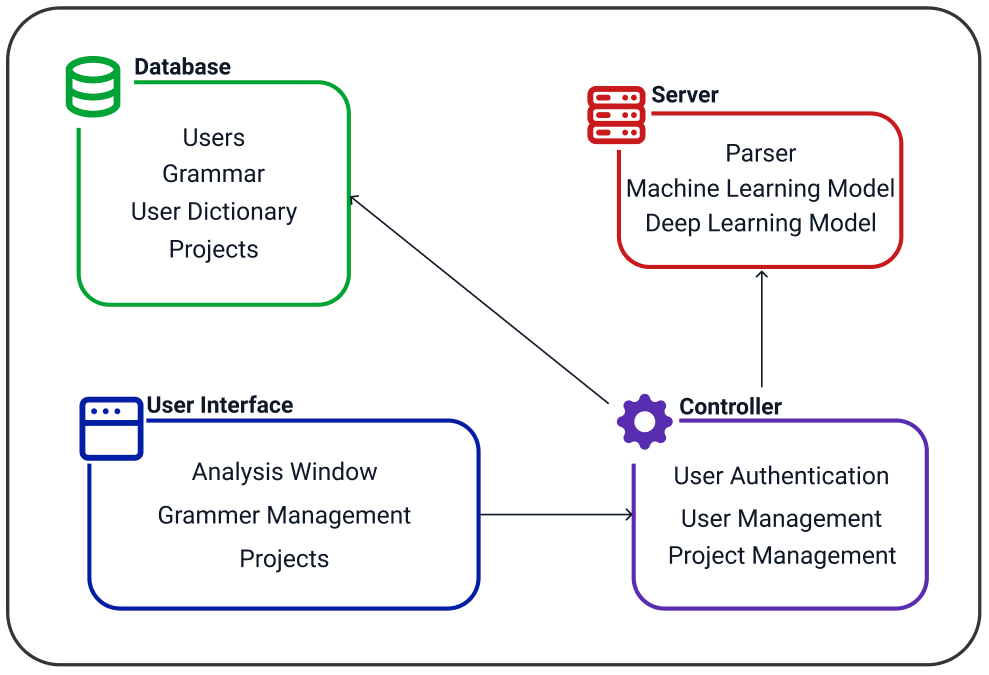
\includegraphics[width=10cm]{Images/System Overview.png}
\subsection{Scope}
The project aims to be used by linguistic professionals to assist them in writing analysis and feature extraction/validation.
\subsection{Project Overview}
\begin{itemize}
    \item Document and project storage.
    \item Analysis server.
    \item User interface.
\end{itemize}

\section{Project Management and Deliverable}
\subsection{Tasks and Time Plan}
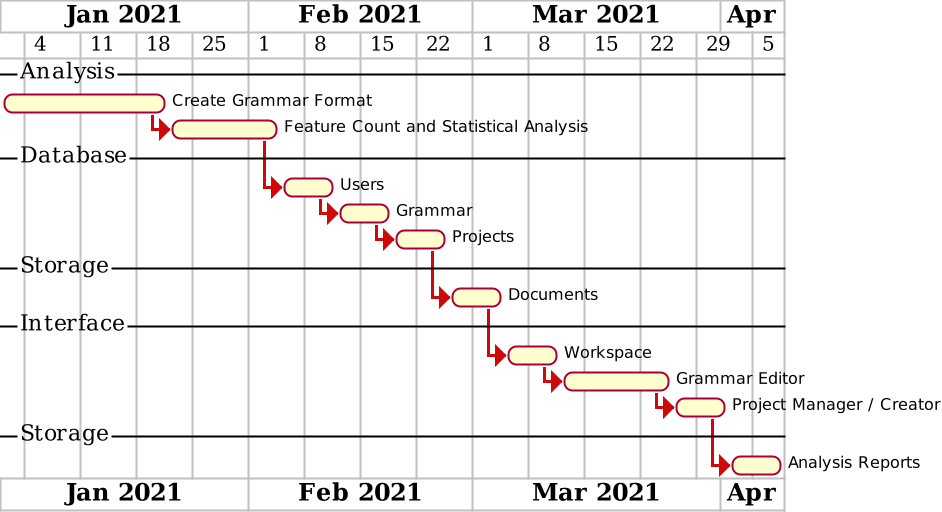
\includegraphics[width=15cm]{Images/gantt.png}

\end{document}
